\documentclass{article}

\usepackage{caption}
\usepackage{subcaption}
\usepackage{graphicx}
\usepackage{tikz}
\usepackage{tikzsymbols}
\usetikzlibrary{calc,patterns,shapes.geometric}
\usepackage{float}

\def\centerarc[#1](#2)(#3:#4:#5){\draw[#1] ($(#2)+({#5*cos(#3)},{#5*sin(#3)})$) arc (#3:#4:#5);}

\pagestyle{empty}
\begin{document}
	\centering
	\begin{figure}[H]
		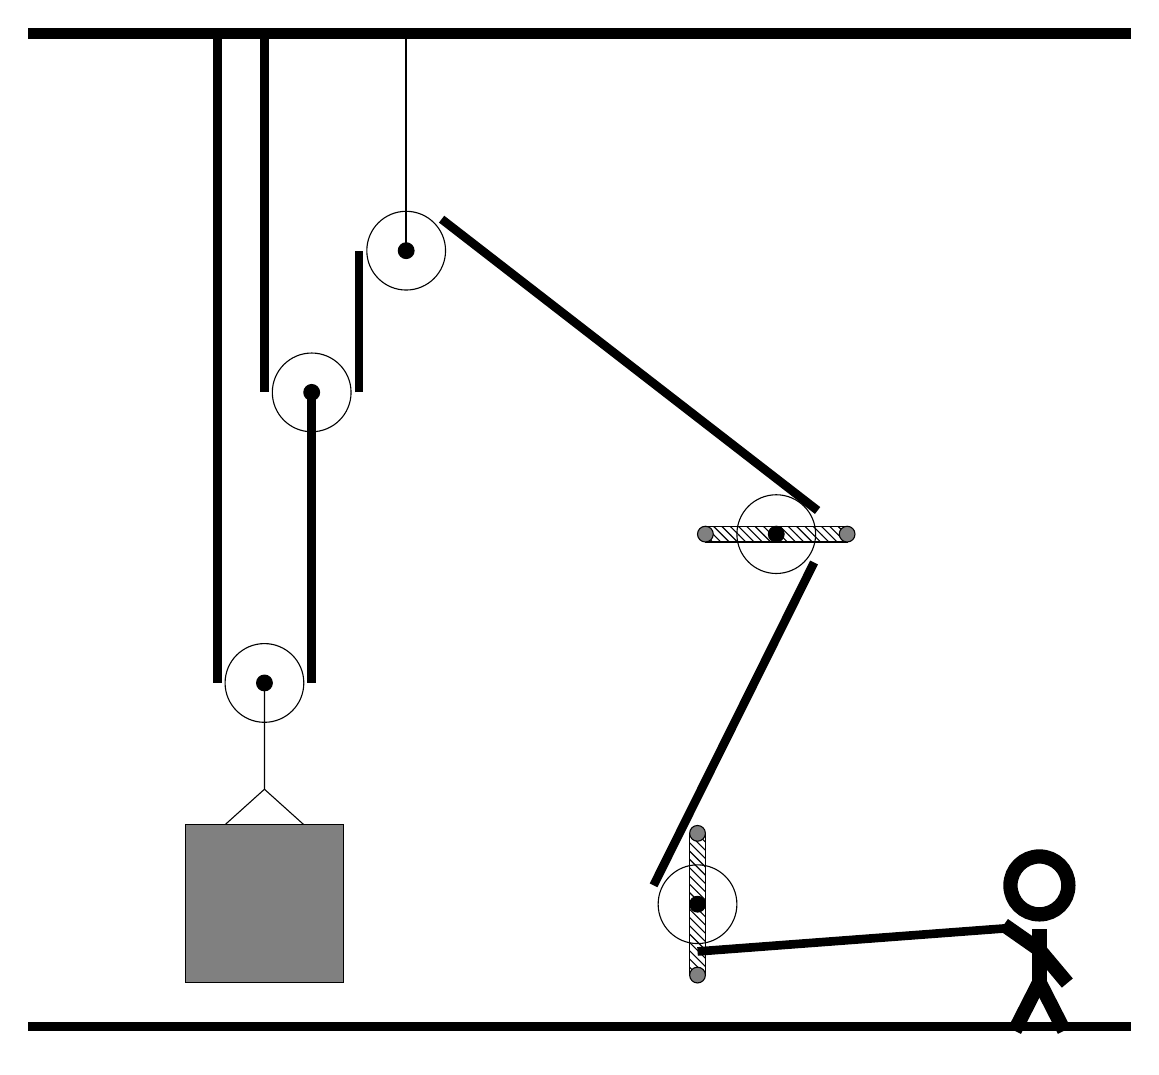
\begin{tikzpicture}
			%%%%% START %%%%%
			\def\a{9}
			\def\radlg{0.5}
			\def\radrp{0.6}
			\def\radsm{0.1}
			\def\yone{0.09*\a}
			\def\xone{1}
			\def\ytwo{\a-0.3*\a}
			\def\xtwo{\xthree+2*\radrp}
			\def\xthree{\xone+\radrp}
			\def\ythree{\a-0.5*\a}
			\def\dx{5.9}
			\def\dy{-1.9}
			\def\dw{1.75mm}
			\def\width{1.1mm}
			\def\bump{0.3}
			\def\ywallone{-2}
			\def\xwallone{\xone+5.5}
			\def\ywalltwo{0.3*\a}
			\def\xwalltwo{\xone+6.5}
			
			\draw[fill=black] (-2,\a) rectangle (12,\a+0.125);
			
			\draw (\xone,\yone) circle (\radlg);
			\draw[fill=black] (\xone,\yone) circle (\radsm);
			
			\draw (\xthree,\ythree) circle (\radlg);
			\draw[fill=black] (\xthree,\ythree) circle (\radsm);
			
			\draw (\xtwo,\ytwo) circle (\radlg);
			\draw[fill=black] (\xtwo,\ytwo) circle (\radsm);
			\draw[thick] (\xtwo,\ytwo) -- (\xtwo,\a);
			
			\draw (\xwallone,\ywallone) circle (\radlg);
			\draw[fill=black] (\xwallone,\ywallone) circle (\radsm);
			\draw[pattern=north west lines, pattern color=black] (\xwallone-0.1,\ywallone+\radrp+\bump) rectangle (\xwallone+0.1,\ywallone-\radrp-\bump); 
			\draw[fill=black!50] (\xwallone,\ywallone+\radrp+\bump) circle (\radsm);
			\draw[fill=black!50] (\xwallone,\ywallone-\radrp-\bump) circle (\radsm);
			
			\draw (\xwalltwo,\ywalltwo) circle (\radlg);
			\draw[fill=black] (\xwalltwo,\ywalltwo) circle (\radsm);
			\draw[pattern=north west lines, pattern color=black] (\xwalltwo-\radrp-\bump,\ywalltwo+0.1) rectangle (\xwalltwo+\radrp+\bump,\ywalltwo-0.1); 
			\draw[fill=black!50] (\xwalltwo-\radrp-\bump,\ywalltwo) circle (\radsm);
			\draw[fill=black!50] (\xwalltwo+\radrp+\bump,\ywalltwo) circle (\radsm);

			\draw (\xone,\yone) -- (\xone,\yone-\a*0.15) -- (\xone-0.5,\yone-\a*0.2) -- (\xone+0.5,\yone-\a*0.2) -- (\xone,\yone-\a*0.15);
			\draw[fill=black!50] (\xone-1,\yone-\a*0.2) rectangle (\xone+1,\yone-\a*0.2-2); 
			
			\draw[line width=\width] (\xone-\radrp,\a) -- (\xone-\radrp,\yone); 
			\centerarc[line width=\width](\xone,\yone)(180:360:\radrp);
			\draw[line width=\width](\xone+\radrp,\yone) -- (\xthree,\ythree);
			\draw[line width=\width] (\xthree-\radrp,\a) -- (\xthree-\radrp,\ythree);
			\centerarc[line width=\width](\xthree,\ythree)(180:360:\radrp);
			\draw[line width=\width](\xthree+\radrp,\ythree) -- (\xtwo-\radrp,\ytwo);
			\centerarc[line width=\width](\xtwo,\ytwo)(35:180:\radrp);
			\draw[line width=\width] (\xtwo+\radrp-\radrp/4,\ytwo+\radrp/1.5) -- (\xwalltwo+\radrp-\radrp/8, \ywalltwo+\radrp/2);
			\centerarc[line width=\width](\xwalltwo,\ywalltwo)(215:135:-\radrp);
			\draw[line width=\width](\xwalltwo+\radrp*0.8,\ywalltwo-\radrp*0.6) -- (\xwallone-\radrp*0.93,\ywallone+0.4*\radrp);
			\centerarc[line width=\width](\xwallone,\ywallone)(-30:100:-\radrp);
			\draw[line width=\width](\xwallone,\ywallone-\radrp) -- (10.5,-2.3);

			\node at (10.8, -2.5) {\Strichmaxerl[10][-35][-50]};
			
			\draw[fill=black] (-2,-3.5) rectangle (12,-3.6);
			%%%%% END %%%%%
		\end{tikzpicture}
	\end{figure}
	
\end{document}